El equipo de red de distribución óptica pasiva (ODN) consiste en un equipo y componentes ubicados entre el OLT (activo) y las instalaciones del cliente (el ONT; activo); este incluye componentes tanto ópticos como no ópticos de la red. Los componentes ópticos forma la red de distribución óptica (ODN) e incluyen empalmes (fusión y mecánicos), conectores, divisores, acopladores WDM, cables de fibra óptica, cordones de conexión y posiblemente terminales de acceso con cables de acceso. Los componentes no ópticos incluyen pedestales, armarios, paneles de conexiones, cajas de empalme y hardware diverso (véase la figura~\figref{fig:ODN_passive}).


\begin{figure}[H]
	\centering
	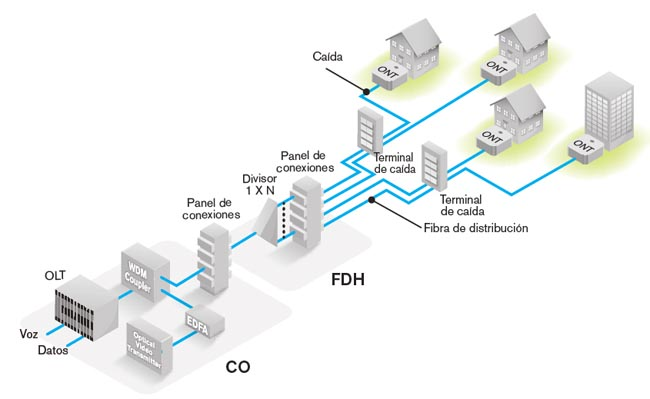
\includegraphics[width=0.75\textwidth]{./img/punto3/Equipo-ODN-pasivo.jpg}
	\caption{Equipo ODN pasivo}
	\label{fig:ODN_passive}
\end{figure}